% THIS DOCUMENT IS FOLLOWS THE VOLERE TEMPLATE BY Suzanne Robertson and James Robertson
% ONLY THE SECTION HEADINGS ARE PROVIDED
%
% Initial draft from https://github.com/Dieblich/volere
%
% Risks are removed because they are covered by the Hazard Analysis
\documentclass[12pt]{article}

\usepackage{booktabs}
\usepackage{tabularx}
\usepackage{hyperref}
\hypersetup{
    bookmarks=true,         % show bookmarks bar?
      colorlinks=true,      % false: boxed links; true: colored links
    linkcolor=red,          % color of internal links (change box color with linkbordercolor)
    citecolor=green,        % color of links to bibliography
    filecolor=magenta,      % color of file links
    urlcolor=cyan           % color of external links
}
\usepackage{amsmath, mathtools}
\usepackage{amsfonts}
\usepackage{array}
\usepackage{amssymb}
\usepackage{graphicx}
\usepackage{colortbl}
\usepackage{xr}
\usepackage{longtable}
\usepackage{xfrac}
\usepackage{float}
\usepackage{siunitx}
\usepackage{caption}
\usepackage{pdflscape}
\usepackage{afterpage}
\usepackage{float}
\usepackage{fullpage}
\usepackage[round]{natbib}

\newcommand{\lips}{\textit{Insert your content here.}}

\input{../Comments}
\input{../Common}

% For easy change of table widths
\newcommand{\colZwidth}{1.0\textwidth}
\newcommand{\colAwidth}{0.13\textwidth}
\newcommand{\colBwidth}{0.82\textwidth}
\newcommand{\colCwidth}{0.1\textwidth}
\newcommand{\colDwidth}{0.05\textwidth}
\newcommand{\colEwidth}{0.8\textwidth}
\newcommand{\colFwidth}{0.17\textwidth}
\newcommand{\colGwidth}{0.5\textwidth}
\newcommand{\colHwidth}{0.28\textwidth}

% Used so that cross-references have a meaningful prefix
\newcounter{defnum} %Definition Number
\newcommand{\dthedefnum}{GD\thedefnum}
\newcommand{\dref}[1]{GD\ref{#1}}
\newcounter{datadefnum} %Datadefinition Number
\newcommand{\ddthedatadefnum}{DD\thedatadefnum}
\newcommand{\ddref}[1]{DD\ref{#1}}
\newcounter{theorynum} %Theory Number
\newcommand{\tthetheorynum}{TM\thetheorynum}
\newcommand{\tref}[1]{TM\ref{#1}}
\newcounter{tablenum} %Table Number
\newcommand{\tbthetablenum}{TB\thetablenum}
\newcommand{\tbref}[1]{TB\ref{#1}}
\newcounter{assumpnum} %Assumption Number
\newcommand{\atheassumpnum}{A\theassumpnum}
\newcommand{\aref}[1]{A\ref{#1}}
\newcounter{goalnum} %Goal Number
\newcommand{\gthegoalnum}{GS\thegoalnum}
\newcommand{\gsref}[1]{GS\ref{#1}}
\newcounter{stretchgoalnum} %Stretch Goal Number
\newcommand{\sgthestretchgoalnum}{STG\thestretchgoalnum}
\newcommand{\sgref}[1]{STG\ref{#1}}
\newcounter{instnum} %Instance Number
\newcommand{\itheinstnum}{IM\theinstnum}
\newcommand{\iref}[1]{IM\ref{#1}}
\newcounter{reqnum} %Requirement Number
\newcommand{\rthereqnum}{R\thereqnum}
\newcommand{\rref}[1]{R\ref{#1}}
\newcounter{nfrnum} %NFR Number
\newcommand{\rthenfrnum}{NFR\thenfrnum}
\newcommand{\nfrref}[1]{NFR\ref{#1}}
\newcounter{lcnum} %Likely change number
\newcommand{\lthelcnum}{LC\thelcnum}
\newcommand{\lcref}[1]{LC\ref{#1}}
\newcounter{ulcnum} %Unlikely change number
\newcommand{\ltheulcnum}{ULC\theulcnum}
\newcommand{\ulcref}[1]{ULC\ref{#1}}

\newcounter{udnum} % User documentation
\newcommand{\ltheudnum}{UD\theudnum}
\newcommand{\udref}[1]{UD\ref{#1}}

\newcounter{trnum} % traninig requirement
\newcommand{\lthetrnum}{TR\thetrnum}
\newcommand{\trref}[1]{TR\ref{#1}}

\newcounter{mnpnum} % traninig requirement
\newcommand{\lthemnpnum}{TR\themnpnum}
\newcommand{\mnpref}[1]{MNP\ref{#1}}

\begin{document}

\title{Software Requirements Specification for \progname: RapidCare} 
\author{\authname}
\date{\today}
	
\maketitle

~\newpage

\pagenumbering{roman}

\tableofcontents
~\newpage

\section*{Revision History}

\begin{tabularx}{\textwidth}{p{3cm}p{2cm}X}
\toprule {\textbf{Date}} & {\textbf{Version}} & {\textbf{Notes}}\\
\midrule
12-10-2025 & 1.0 & Rev 0\\
06-01-2025 & 1.1 & Pranav Updated: TA feedback parts (Removed implementation details, fixed wordings, Traceability Matrix)\\
19-03-2025 & 1.2 & Template Update \\
24-03-2025 &1.2 & Added Missing sections \\
31-03-2025 & 1.2 & Pranav added formal specification, ammended requirements, updated trace matrix. \\
31-03-2025 & 1.2 & Inreet Amended section to include external knowledge and impact \\


\bottomrule
\end{tabularx}

~\\

~\newpage

\section{Introduction}

\subsection{Purpose of Document} \label{sec_PurposeOfDocument}
The purpose of this document is to provide a comprehensive description of the requirements for a software application that aims to streamline the healthcare documentation process aimed to be run as a web application. This document will be used as a contract in a sense between the team and the client who intends to use this application. This document will allow for an in-depth description of the software's functionality, performance, and other non-functional requirements. Additionally, it will outline common use-cases under which the software will be used. This will in turn provide a direction to the developers such that they will be empowered to creating the right product as this document will contain various stakeholders' requirements. Along with development direction, this document will be a direct reference for all of the stakeholders to understand the product's scope, functionality, and limitations.

\subsection{Characteristics of Intended Reader} \label{sec_IntendedReader} 

The intended readers of this SRS document include project managers, software developers, testing engineers, and stakeholders directly involved in the design and implementation of the software system. Project managers and testing engineers would be directly involved in the development and testing process. They would generally have an education in computer science along with experience in software design, web or mobile development, and software testing. Project managers generally have experience in managing software projects and knowledge of software development processes. Stakeholders like doctors and nursing staff would have domain knowledge and could provide insights to understand the clinical workflow and documentation process. 


\section{Purpose of the Project}

\subsection{User Business}

The healthcare industry in Canada is facing significant challenges. After talking to multiple stakeholders, we discovered that the major reason behind this is documentation overhead and inefficient workflows. Healthcare professionals spend a major portion of their time on documentation tasks. This in turn leaves them with less time to actually provide care to patients. This contributes to longer wait times, reduced patient throughput, and increased stress on healthcare workers.\\
The current EHR systems are often difficult to navigate and require manual data entry, which is time-consuming and prone to errors. Moreover, the EHR systems with speech-to-text transcription are not very accurate and require a lot of review from the users. These EHR systems are quite expensive and cannot be afforded by smaller practices. Therefore, healthcare professionals need a more efficient way to document patient interactions and health data which is cost-effective and also extends the functionality of the current EHR systems.\\
This project aims to address these issues by providing a healthcare documentation system that leverages speech recognition and ML to streamline the documentation process. Along with real-time transcription and classification of the text, the system will also be able to provide diagnostic and treatment plan suggestions to reduce cognitive load and improve accuracy. This will reduce the time spent on administrative tasks, allowing healthcare professionals to focus more on patient care while maintaining accurate and comprehensive medical records.\\

\subsection{Goals of the Project}

The goals for this project are as follows:

\begin{table}[H]
  \centering
  \begin{tabular}{p{4cm} p{4cm} p{4cm}}
      \toprule
      \textbf{Goal} & \textbf{Explaining} & \textbf{Reasoning} \\
      \midrule
      Use voice to fill in medical documentation (charts, files, etc.) & The app will record conversations and automatically turn them into medical notes and charts. & This will save doctors time by automating paperwork, letting them focus more on patients. \\
      \midrule
      Reduce documentation overhead time.  & Through tracking the whole patient journey in the app, we look to reduce the overhead of triaging, clinical documentation, and other registrations.  & This helps hospital healthcare professionals focus on care and lowers the time taken through registration for hospital staff. \\
      \midrule
      Automated diagnosis suggestions.  & Use AI to suggest possible diagnoses based on what the doctor and patient discuss.  & This will help doctors make faster, more accurate diagnoses, especially in tricky cases. \\
      \midrule
      Automated treatment plan suggestions. & Based on diagnosis and patient data provide treatment plan suggestions. & This will help doctors fill out their charts faster. \\
      \bottomrule
  \end{tabular}
\end{table}

\section{Stakeholders}

\subsection{Client}
The primary client for this project are healthcare institutions such as hospitals and clinics. These institutions will benefit from the project as it will help in streamlining the documentation process, reducing administrative overhead, and enhancing the quality of patient care.

\subsection{Customer}
The primary customer of the project are healthcare professionals, specifically those involved in patient documentation, including doctors, nurses, and other clinical administrative staff. The project will provide a user-friendly system that allows for efficient data entry and retrieval, as well as accurate transcription of patient interactions. The system will minimize the time spent on documentation, allowing them to focus more on patient care.

\subsection{Other Stakeholders}
\begin{itemize}
  \item \textbf{Society:} Society is a major stakeholder in this project. The healthcare institutions such as hospitals and clinics are a part of users group within the society that will be benefited with improved efficiency, effective staff management, and reduction in cost. This project will significantly impact various aspects like health, safety, and cultural diversity of society. By reducing documentation overhead, healthcare professionals can spend more time with patients, leading to better quality of care. This will help reduce emergency room wait times, ultimately improving public health outcomes. The system will meet all accessibility standards, use appropriate medical terminology, and does not use biased language to accommodate users with diverse cultural backgrounds. Accurate documentation and diagnostic suggestions will help reduce medical errors and improve patient safety.

  \item \textbf{Regulatory Bodies:} These are the organizations that set standards for healthcare technology and data protection. They are concerned with compliance to regulations such as PIPEDA and other relevant laws.
\end{itemize}

\subsection{Hands-On Users of the Project}
\begin{itemize}
  \item\textbf{Healthcare Professionals:} These include the hospital staff such as Doctors, nurses etc, who will use the system.
  \item\textbf{Healthcare Network Employees:} These are the people employed in the organization who keeps records of all hospital facilities, their staff members and authenticates the healthcare professionals so that they are able to use the system. 
\end{itemize}

\subsection{Personas}
\begin{itemize}
    \item \textbf{Healthcare Professional: Dr. Virat} - Dr. Virat works in the emergency department at Brampton Hospital. He frequently uses EHR systems to document clinical notes and manage patient records. However, he feels that most of his time is spent recording notes. He wishes for a system that could speed up this process and allow him to focus more on direct patient care and serve more patients throughout the day.
    \item \textbf{Nurse: Anushka} - Anushka is a registered nurse who relies on the system to access patient information quickly and update records during patient triage. She often feels stressed due to increased patient volume and long hours of shift due to inefficient staff management at her hospital.
    \item \textbf{Patient: John} - John is a working professional who recently visited the emergency department for a sprained ankle. He had to wait 13 hours in the emergency room due to high patient volume and inefficient documentation process. He expects the system to reduce wait times.
\end{itemize}

\subsection{Priorities Assigned to Users}
\begin{itemize}
    \item \textbf{High Priority:} Healthcare professionals have the highest priority as they are direct users of the system and are directly involved in patient care and operational efficiency.
    \item \textbf{Medium Priority:} Healthcare network administrators have medium priority as they are responsible for managing user access and ensuring data integrity but do not interact with the system as frequently as healthcare professionals.
    \item \textbf{Low Priority:} All other stakeholders including patients and regulatory bodies have low priority. While they benefit from the system's functionality, they are not direct users and rely on healthcare professionals to manage their information.
\end{itemize}

\subsection{User Participation}
User participation is vital for the design, development, and acceptance testing of the system. Users like healthcare professionals can provide feedback during the design and testing phases to ensure the system meets their critical needs. This will help in gathering insights on usability and functionality, allowing for iterative improvements to the system.

\subsection{Maintenance Users and Service Technicians}
System administrators and IT staff will be responsible for maintaining the system. They would be responsible to provide assistance to the users and troubleshoot any technical issues that may arise ensuring that the system remains functional. 

\section{Mandated Constraints}

\subsection{Solution Constraints}
The following fundamental constraints govern the core functionality of the system:

\begin{table}[H]
\centering
\begin{tabular}{|p{6cm}|p{6cm}|}
\hline
\textbf{Constraint} & \textbf{Rationale} \\
\hline
The system must adhere to healthcare regulations. & Mandatory for handling patient health information and ensuring the confidentiality and security of patient data. \\
\hline
The system must maintain PIPEDA compliance for all patient data. & Essential for protecting patient privacy and meeting Canadian healthcare data protection standards. \\
\hline
The system must comply with Canada's Privacy Law and all applicable healthcare data protection regulations. & Required to ensure legal compliance and protect sensitive medical information. \\
\hline
\end{tabular}
\caption{Solution Constraints}
\label{tab:solution_constraints}
\end{table}

\subsection{Implementation Environment of the Current System}
The system must operate within these environmental parameters:

\begin{table}[H]
\centering
\begin{tabular}{|p{6cm}|p{6cm}|}
\hline
\textbf{Constraint} & \textbf{Rationale} \\
\hline
Must function with standard clinic recording devices. & Users should not incur extra hardware costs. \\
\hline
The system must be accessbile on standard web browsers and working stations. & Ensures accessibility across different platforms. \\
\hline
\end{tabular}
\caption{Implementation Environment Constraints}
\label{tab:implementation_constraints}
\end{table}

\subsection{Partner or Collaborative Applications}
Integration with external systems must comply with:

\begin{table}[H]
\centering
\begin{tabular}{|p{6cm}|p{6cm}|}
\hline
\textbf{Constraint} & \textbf{Rationale} \\
\hline
Cloud hosting services shall guarantee 99.9\% uptime. & Necessary to meet the robustness requirements for healthcare systems. \\
\hline
Must support integration with existing EHR systems. & Ensures seamless data exchange. \\
\hline
\end{tabular}
\caption{Partner Application Constraints}
\label{tab:partner_constraints}
\end{table}

\subsection{Off-the-Shelf Software}
Third-party components must meet these standards:

\begin{table}[H]
\centering
\begin{tabular}{|p{6cm}|p{6cm}|}
\hline
\textbf{Constraint} & \textbf{Rationale} \\
\hline
All third-party libraries must be actively maintained with security updates. & Essential to meet security and maintainability. \\
\hline
\end{tabular}
\caption{Off-the-Shelf Software Constraints}
\label{tab:off_the_shelf_constraints}
\end{table}

\subsection{Anticipated Workplace Environment}
The system must accommodate these workplace conditions:

\begin{table}[H]
\centering
\begin{tabular}{|p{6cm}|p{6cm}|}
\hline
\textbf{Constraint} & \textbf{Rationale} \\
\hline
The system must be functional in noisy hospital and clinical environments. & Ensures reliable audio capture in real conditions. \\
\hline
\end{tabular}
\caption{Workplace Environment Constraints}
\label{tab:workplace_constraints}
\end{table}

\subsection{Schedule Constraints}
Project timelines must respect these mandatory sequences:

\begin{table}[H]
\centering
\begin{tabular}{|p{6cm}|p{6cm}|}
\hline
\textbf{Constraint} & \textbf{Rationale} \\
\hline
The voice recognition core must be finalized before UI integration. & UI design depends on transcription capabilities as per usability requirements. \\
\hline
Comprehensive testing must be conduted before each deployment iteration. & Ensures system reliability and accuracy. \\
\hline
\end{tabular}
\caption{Schedule Constraints}
\label{tab:schedule_constraints}
\end{table}

\subsection{Budget Constraints}
Financial limitations for the project include:

\begin{table}[H]
\centering
\begin{tabular}{|p{6cm}|p{6cm}|}
\hline
\textbf{Constraint} & \textbf{Rationale} \\
\hline
Total project expenditures shall not exceed \$50. & Course-mandated budget cap for all development and testing. \\
\hline
\end{tabular}
\caption{Budget Constraints}
\label{tab:budget_constraints}
\end{table}

\subsection{Enterprise Constraints}
Organizational policies impose these requirements:

\begin{table}[H]
\centering
\begin{tabular}{|p{6cm}|p{6cm}|}
\hline
\textbf{Constraint} & \textbf{Rationale} \\
\hline
All code changes require peer review before deployment. & Ensures code quality and reliability. \\
\hline
\end{tabular}
\caption{Enterprise Constraints}
\label{tab:enterprise_constraints}
\end{table}

\section{Naming Conventions and Terminology}

\subsection{Glossary of All Terms, Including Acronyms, Used by Stakeholders
involved in the Project}
The following is the glossary for this document:
\begin{itemize}
  \item \textbf{System:} The intended solution/product.
  \item \textbf{User:} A person who will use the product.
  \item \textbf{Healthcare Professional:} A doctor, nurse, and other healthcare professional who will be using the product.
  \item \textbf{Patient:} Any person who is receiving medical treatment.
  \item \textbf{Healthcare Network:} An organisation that has group of hospitals or clinics and will use the system.
\end{itemize}

\begin{tabular}{l l} 
  \toprule    
  \textbf{symbol} & \textbf{description}\\
  \midrule 
  A & Assumption\\
  G & Goals\\
  UI & User Interface\\
  UX & User Experience\\
  PIPEDA & Personal Information Protection and Electronic Documents Act\\
  STG & Stretch Goals\\
  FR & Functional Requirement\\
  NFR & Non-functional Requirement\\
  LC & Likely Change\\
  ULC & Unlikely Change\\
  SRS & Software Requirements Specification\\
  EHR & Electronic Healthcare Record\\
  SOAP & Subjective Objective Assessment Plan \\
  ML & Machine Learning \\
  API & Application Programming Interface \\
  TR & Trainig Requirement \\
  UD & User Documentation Requirement \\
  MNP & Migration to new Product Requirement \\
  \bottomrule
\end{tabular}\\

\section{Relevant Facts And Assumptions}

\subsection{Relevant Facts}
\begin{itemize}
  \item The healthcare system in Canada faces significant challenges due to documentation overhead.
  
  \item The current EHR systems mostly use manual data entry and basic speech-to-text functionality. This impacts the efficiency of the workflow and is prone to errors.
  
  \item The NLP techniques and speech recognition software have made significant advancements in recent years. 
  
  \item These technologies can be adapted to improve accuracy, provide diagnostic and treatment plan suggestions, and improve the efficiency of healthcare workflows. 
  
  \item The healthcare industry has strict regulations regarding patient data privacy and security.
\end{itemize}

\subsection{Business Rules}
\begin{itemize}
  \item Access to patient records must be strictly controlled based on user roles and permissions.
  
  \item The system must comply with all relevant healthcare data protection regulations, including PIPEDA and other privacy laws.
  
  \item Any modifications to the codebase must be accompanied by a review from peers to meet the standard coding standards.
  
  \item The project must implement a CI/CD pipeline to ensure that all changes are validated before integration.

  \item The system must be scalable to accommodate large datasets and multiple users accessing the system simultaneously.
\end{itemize}

\subsection{Assumptions}

\begin{itemize}
  \item[A\refstepcounter{assumpnum}\theassumpnum \label{A_reliableInternet}:] \textbf{Reliable Internet Connection:} We assume that the user has a reliable internet connection throughout their operational hours.
  \item[A\refstepcounter{assumpnum}\theassumpnum \label{A_sufficientHardware}:] \textbf{Sufficient Hardware Accessories:} We are assuming that the user has the required hardware devices such as monitors, iPads etc. to access the system.
  \item[A\refstepcounter{assumpnum}\theassumpnum \label{A_patientConsent}:] \textbf{Patient's Consent:} We also assume that medical staff will obtain patients' consent when required.  
\end{itemize}


\section{The Scope of the Work}

\subsection{The Current Situation}
Ontario is facing an extreme shortage of family doctors, with the number of patients without one jumping by 600,000 to 2.5 million which is a growing number [1]. This situation is only to get worse as predicted by the Ontario Medical Association [2]. As a result, people find themselves going to the ER with coughs and colds and flooding the ER causing massive wait times which ends in patients even resulting in leaving without being seen [3]. A massive part of the wait time is due to the overhead of documentation tasks. Doctors, healthcare professionals, and support staff find themselves spending most of their time on documentation which overall slows the pipeline of patients tremendously.

\subsection{The Context of the Work}

Through this project we aim to develop a solution that will address key niche problems through customizability and add features of critical need that do not already exist in existing solutions. This will allow healthcare networks to centralize the data of their hospitals and increase the staff productivity.\\

\noindent This product has been conceived by the group members based on elicitation. Through interviews and discussion the problem of documentation overhead was found. This is the problem to be solved for the capstone course SFWRENG 4G06.

\begin{figure}[H]
  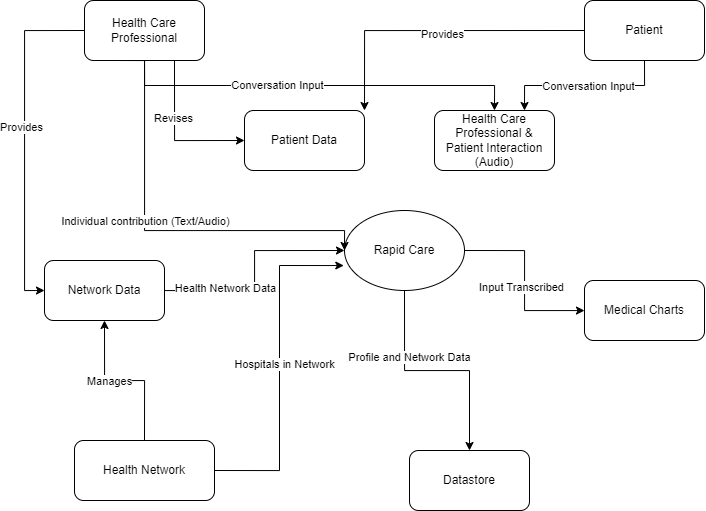
\includegraphics[width=0.8\textwidth]{System_Context.png}
  \caption{This is the System Context diagram for this scenario.}
  % \label{fig:Use-Case Diagram}
\end{figure}

\begin{itemize}
  \item \textbf{Inputs:}
  \begin{itemize}
    \item \textbf{Doctor-Patient Conversation} -- The conversation between the doctor and the patient is recorded using the recording tool.
    \item \textbf{Medical Prediction Context} -- A comprehensive knowledge of common diseases and the associated medicines is served as input for the model to predict the diagnosis and treatment plans.
    \item \textbf{Text Field Input} -- Text field entries are utilized as input parameters provided by the user for various data processing operations such as filling out patient data, creating consultation notes, etc.    
  \end {itemize}
  \item \textbf{Outputs:}
  \begin{itemize} 
    \item \textbf{Transcribed Text} -- The audio from healthcare professional and patient conversation is transcribed into text.
    \item \textbf{Auto-filled documents} -- The transcribed text is further classified into relevant categories to autofill the charts with patient's medical information.
    \item \textbf{Predicted Diagnosis and Plan} -- Classified data is used to provide diagnosis and the treatment plan based on the context about common diseases and associated diagnosis.  
  \end{itemize}
  \item \textbf{User Responsibilities:}
  \begin{itemize}
    \item Record audio.
    \item Amend or delete documentation as needed.
    \item Maintain existing data, and journey tracks.
  \end{itemize}
  \item \textbf{System Responsibilities:}
  \begin{itemize}
    \item Accurately transcribe audio into text and classify it.
    \item Accurate mapping of patient journey in application.
  \end{itemize}

\item{\textbf{Expected Benefits:}}

\begin{itemize}
  \item Reduced documentation overhead time
  \item Increased patient throughput
  \item Improved patient care
  \item Increased doctor and healthcare professional satisfaction
\end{itemize}
\end{itemize}


\subsection{Work Partitioning}
\lips

The work partitioning for this project was done as follows:

\begin{enumerate}

  \item \textbf{Research and Data Collection:} Research and gather a dataset of the current diseases and associated medicines to train and test the diagnosis and treatment plan prediction models.\\
  \item \textbf{Model Development:} Develop a machine learning model which is trained on the gathered dataset of current diseases and associated medicines, to assist in the diagnosis of the patient and prediction of potential treatment options.\\
  \item \textbf{Unit Testing and Validation:} Conduct unit testing on the modules with various test cases to validate the performance and accuracy of the system. This will also help to ensure that the existing code implementation remains intact after the code is given various inputs.\\
  \item \textbf{Documentation:} Document the system's architecture, performance and corresponding results after unit testing is performed on each module.\\  

\end{enumerate}

\subsection{Specifying a Business Use Case (BUC)}

\textbf{Main Usage Scenario: Documenting a Patient Consultation}

\begin{itemize}
  \item\textbf{Use Case:} UC2, UC3
  \item\textbf{Primary Actor:} Healthcare professional (such as a medical doctor or a nurse)
  \item\textbf{Precondition:} The user has been successfully authenticated, logged into the system and has patient's profile is created. The basic information such as name, contact information, and history is prefilled.
  \item\textbf{Trigger:} The user will initiate dictation.
  \item\textbf{Main Success Scenario:}
  \begin{itemize}
    \item The user will initiate dictation.
    \item The system will convert audio to text in real-time.
    \item The user will press stop button.
    \item The user reviews the transcribed notes. 
    \item The system has accurately transcribed the audio to text without any inaccuracies.
    \item The user selects the submit button after review. 
  \end{itemize}
  \item\textbf{Secondary Success Scenario:}
  \begin{itemize}
    \item The system has produced some inaccuracies in the transcribed text.
    \begin{itemize}
      \item The user selects the edit button.
      \item The system prompts user to edit the text.
      \item The user manually edits the transcribed text.
    \end{itemize} 
  \end{itemize}
  \item\textbf{Success Postcondition:}
  \begin{itemize}
    \item The notes are successfully saved in patient database and changes are reflected in the user interface.
  \end{itemize}
\end{itemize}

\section{Business Data Model and Data Dictionary}
\subsection{Business Data Model}

The essential objects/entities for this project and their relations are outlined below. It can be noted that the entities along with their relationships follow the usual model of a hospital based on discussions with our supervisor.

\begin{figure}[H]
  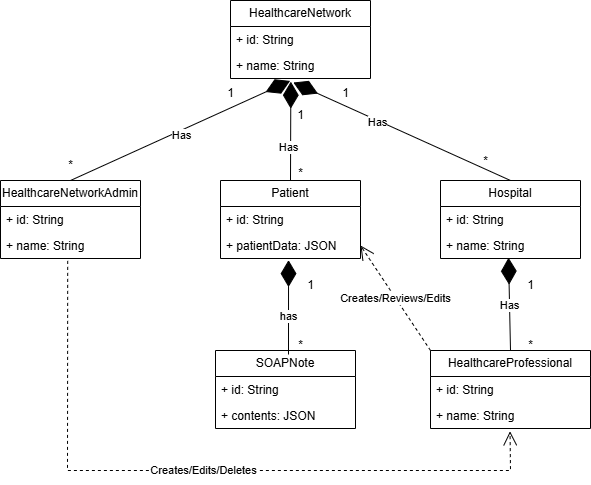
\includegraphics[width=0.8\textwidth]{DataModel.png}
  \caption{This is the Buisness Data Model.}
  % \label{fig:Use-Case Diagram}
\end{figure}

\subsection{Data Dictionary}
\begin{center}
\begin{tabular}{ | m{15em} | m{20em}| m{5em} | } 
  \hline
  \textbf{Name}& \textbf{Content} & \textbf{Type} \\ 
  \hline
  HealthcareNetwork & Represents a healthcare network. & class \\ 
  \hline
  HealthcareNetworkAdmin & Represents a administrator at a healthcare network. & class \\ 
  \hline
  Patient & Represents a patient recieving care at a hospital with in a healthcare network. & class \\ 
  \hline
  Hospital & Represents a hospital in a healthcare network. & class \\ 
  \hline
  SOAPNote & Represents a subjective, objective, assessment, and plan that is attained through a doctor - physician conversation. This includes signs, symptoms and plans.& class \\ 
  \hline
  HealthcareProfesional & Represents a healthcare proffesional working at a hospital with in a given healthcare network.& class \\ 
  \hline
\end{tabular}
\end{center}
\section{The Scope of the Product}
\subsection{Product Boundary}
The scope of this project can be be split into the following:

\begin{itemize}
  \item \textbf{Out of Scope:}
  \begin{itemize}
    \item The system will not be responsible for patient scheduling, billing, or other administrative tasks.
    \item The system will not include development of any hardware components. All needed peripherals will be assumed as apart of the runtime environment.
  \end{itemize}
  \item \textbf{Typical Values of Input}
  \begin{itemize}
    \item The primary input mode will be audio, allowing for transcription and segmentation of conversations.
    \item The other input is typing through a keyboard to amend or edit any documentation.
    \item Standard office environment is expected, with standard computer equipment (i.e. mice, keyboards, internet).
  \end{itemize}
\end{itemize}

\subsection{Product Use Case Table}
% not completed

\begin{tabular}{ | p{3cm} | p{3cm} | p{3cm} | p{3cm} | p{3cm} | }
  \hline
  \textbf{PUC No} & \textbf{PUC Name} & \textbf{Actor} & \textbf{Input} & \textbf{Output}  \\ \hline
  1 & Login/Register & Healthcare professional & Login credentials & Access to System \\ \hline
  2 & Recording Clinical Notes & Healthcare professional & Conversation with the patient & System displays transcripted text \\ \hline
  3 & Diagnostic Suggestions & Healthcare professional & Submits transcripted text & Potential diagnostic suggestions based on the transcripted text \\ \hline
  4 & Create Patient Profile & Healthcare professional & Provides patient details in the required fields & Patient profile is created after submission \\ \hline 
\end{tabular}
\captionof{table}{Product Use Case Table}

\subsection{Individual Product Use Cases (PUC's)}

\begin{itemize}
  \item\textbf{UC1 Login:}
  \begin{itemize}
    \item The user accesses the system using an internet browser.
    \item The user enters valid credentials on the log in page.
    \item The user selects the login button.
    \item The user lands on the default dashboard.
  \end{itemize}
  \item\textbf{UC2 Recording Clinical Notes:}
  \begin{itemize}
    \item The user accesses patient's record.
    \item The user initiates dictation.
    \item The user dictates the notes and hit the stop button.
    \item The user reviews the transcribed text.
    \item The user selects the submit button.
  \end{itemize}
  \item\textbf{UC3 Diagnostic Suggestions:}
  \begin{itemize}
    \item The user submits the transcribed text.
    \item The user reviews the potential diagnostic suggestions.
    \item The user accepts or rejects suggestions.
  \end{itemize}
  \item\textbf{UC4 Create Patient Profile:}
  \begin{itemize}
    \item The user log into the system.
    \item The user selects the 'create a new record' button.
    \item The user provide input for the required fields.    
    \item The user selects the submit button.
  \end{itemize}
\end{itemize}

\begin{figure}[H]
  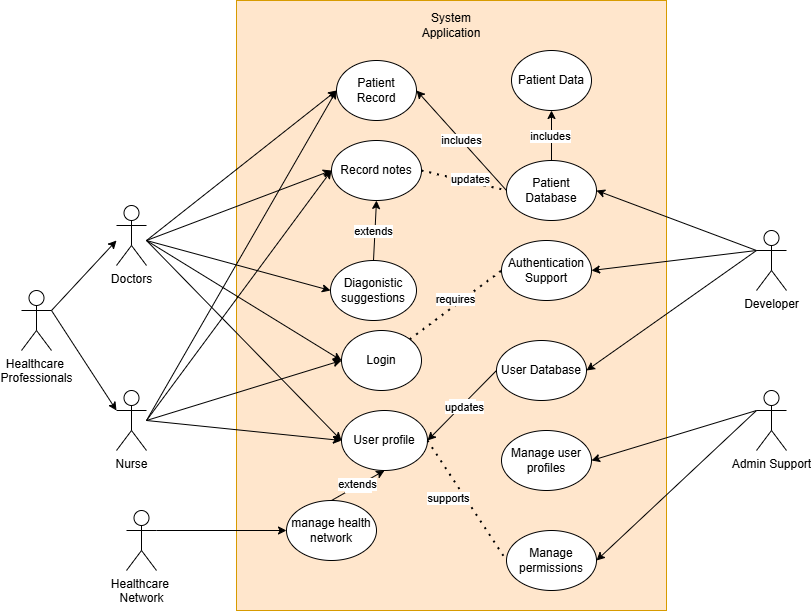
\includegraphics[width=0.8\textwidth]{use-case.drawio.png}
  \caption{This is the use-case diagram for this scenario.}
  \label{fig:Use-Case Diagram}
\end{figure}

\subsection{System Boundaries}
\begin{itemize}
  \item The system will not be responsible for patient scheduling, billing, or other administrative tasks.
  \item The system will not include development of any hardware components. All needed peripherals will be assumed as apart of the runtime environment.
\end{itemize}

\section{Functional Requirements}

\noindent \begin{itemize}

  \item [FR\refstepcounter{reqnum}\thereqnum \label{FR_addHealthNetwork}:] 
  
  \textbf{Requirement:} The system should allow a healthcare network to be onboarded to the system.
  
  \textbf{Rationale:} Rapid care is an organizational tool, where networks can register their various hospitals, and in turn add the corresponding health care professionals. When the networks want to register, the app needs to be able to add the network to the database along with the relevant staff profiles etc.
  
  \textbf{Fit Criterion:} The network data and profiles are fully added to the database. This could be verified by returning the valid entries from the patient database.
  
  \textbf{Dependencies:} N/A
  
  \textbf{Monitored and Controlled Variables:} N/A
  
  \textbf{Performance Requirements:} 
  \begin{itemize}
    \item The system should update the entries with the latency of 1 second.
    \item After user input is taken the system only adds valid entries to the database and prevents any data leaks.
  \end{itemize}
  
  \textbf{Hardware Requirements:} 
  \begin{itemize}
    \item Workstations and other peripherals to access the system.
  \end{itemize}
  
  \textbf{Software Requirements:} 
  \begin{itemize}
    \item Database management system to store health network data.
    \item Internet browser to access the application.
  \end{itemize}
  
  \textbf{Normal Behavior:} 
  \begin{itemize}
    \item All input data is validated as being entered into the system.
    \item Once all required fields are completed the user selects the submits the information and the network is added successfully to the system.
    \item The process should have a low turnover time such that health networks will not have to spend a long time waiting to use the system.
  \end{itemize}
  
  \textbf{Undesired Event Handling:} 
  \begin{itemize}
    \item The user may enter invalid input data. The system should display appropriate error messages. 
    \item The system should have constraints to restrict the user from submitting, unless all required fields are completed and have valid input data. 
    \item When the database is overloaded with requests, appropriate error messages should be delayed. 
    \item The updates will be queued to prevent this in the future, data resources will be scaled just so that the calls are faster.
  \end{itemize}
  
  
  \item[FR\refstepcounter{reqnum}\thereqnum \label{FR_removeHealthNetwork}:]  
  
  \textbf{Requirement:} The system should allow health network to remove itself from the system.
  
  \textbf{Rationale:} 
  When health networks close and want to pivot to another documentation tool their data and profiles must be deleted. Therefore, there is a requirement for functionality that allows organizations to deregister and have their data deleted.
  
  \textbf{Fit Criterion:} 
  The network data and profiles are fully deleted from the database. This could be verified by returning the valid entries from the patient database.
  
  \textbf{Dependencies:} FR\ref{FR_addHealthNetwork} 
  
  \textbf{Monitored and Controlled Variables:} N/A
  
  \textbf{Performance Requirements:} 
  \begin{itemize}
    \item The removal process must be easy to complete with a latency of 1 second. 
    \item The system should be able to identify the correct record to delete. 
    \item The system should delete the correct record without affecting the rest of the database. 
  \end{itemize}
  
  \textbf{Hardware Requirements:} 
  \begin{itemize}
    \item Workstations and other peripherals to access the system.
  \end{itemize}
  
  \textbf{Software Requirements:}
  \begin{itemize}
    \item Access to health network database.
    \item Internet browser to access the application.
  \end{itemize}
  
  \textbf{Normal Behavior:}
  \begin{itemize}
    \item Network is successfully removed from database with low turnover time such that health networks will not have to spend a long time waiting for their data to be deleted.
  \end{itemize}
  
  \textbf{Undesired Event Handling:}
  \begin{itemize}
    \item If the system fails to delete the health network due to a system error, the system should display an appropriate error message. 
    \item When the database is overloaded with requests, the operation to delete all the hospital data will be queued as the next action in line.
  \end{itemize}
  
  
  \item[FR\refstepcounter{reqnum}\thereqnum \label{FR_UpdateHealthNetwork}:]
  
  \textbf{Requirement:} The healthcare network should be able to update its organizational and hospital information.
  
  \textbf{Rationale:} The healthcare network will update its own organizational changes. This will include creating and maintaining the staff present as well as the hospitals in the network.
  
  \textbf{Fit Criterion:} The healthcare network data will be up to date with its current state (i.e. number of hospitals, staff etc.), the data's recency will depend on the networks need. 
  
  \textbf{Dependencies:} FR\ref{FR_addHealthNetwork}
  
  \textbf{Monitored and Controlled Variables:} N/A
  
  \textbf{Performance Requirements:} 
  \begin{itemize}
    \item The updating process of healthcare networks should be quick and easy so that healthcare professionals remain up to date with the facility information, operational data, healthcare professional data, and patient data.
    \item Under a standard load the request should be fulfilled within 1 second.
  \end{itemize}
  
  \textbf{Hardware Requirements:} 
  \begin{itemize}
    \item Workstations and other peripherals to access the system.
  \end{itemize}
  
  \textbf{Software Requirements:} 
  \begin{itemize}
    \item Internet browser to access the application.
  \end{itemize}
  
  \textbf{Normal Behavior:}
  \begin{itemize}
    \item Network is updated in the database without any leaks or latency.
    \item Normal behavior will be seen as updated reflected on the front-end and backend of the system.
  \end{itemize} 
  
  \textbf{Undesired Event Handling:} 
  \begin{itemize}
    \item When the health network data is being updated and the database is overloaded with requests, then updates will be queued.
  \end{itemize}
  
  \item[FR\refstepcounter{reqnum}\thereqnum \label{FR_AddHealthProfessional}:]
  
  \textbf{Requirement:} The system should allow healthcare network administrators to add healthcare professionals to the system.
  
  \textbf{Rationale:} When new healthcare professionals join the healthcare network, their information is to be added to the system for authentication purposes. This will include adding a list of hospital staff members to the network.
  
  \textbf{Fit Criterion:} The healthcare professional's data will be up to date in the system so that they can get authenticated without any delay. 
  
  \textbf{Dependencies:} N/A 
  
  \textbf{Monitored and Controlled Variables:} N/A
  
  \textbf{Performance Requirements:} 
  \begin{itemize}
    \item The addition process should be quick and easy to ensure that all professionals can access the database without any interruptions, with a minimum uptime of 99.5\%.
  \end{itemize}
  
  \textbf{Hardware Requirements:} 
  \begin{itemize}
    \item Workstations and other peripherals to access the system.
  \end{itemize}
  
  \textbf{Software Requirements:} 
  \begin{itemize}
    \item Internet browser to access the database.
  \end{itemize}
  
  \textbf{Normal Behavior:}
  \begin{itemize}
    \item Data is added to the database without any leaks or latency. Normal behavior will be seen as updated are reflected in database and UI of the system.
  \end{itemize} 
  
  \textbf{Undesired Event Handling:}
  \begin{itemize}
    \item When the healthcare professional's data is being added and the database is overloaded with requests, then updates will be queued.
  \end{itemize} 
  
  \item[FR\refstepcounter{reqnum}\thereqnum \label{FR_RemoveHealthProfessionals}:] 
  
  \textbf{Requirement:} The system should allow healthcare network administrators to remove healthcare professionals from the system. 
  
  \textbf{Rationale:} Sometimes a healthcare professional decides to change the area of service or leaves the organization and retires. Therefore, there is a need for functionality that allows to remove them from the system.
  
  \textbf{Fit Criterion:} The healthcare professional is successfully removed from the system, this will be verified by the fact that they are not present in the databases. 
  
  \textbf{Dependencies:} FR\ref{FR_AddHealthProfessional}
  
  \textbf{Monitored and Controlled Variables:} N/A
  
  \textbf{Performance Requirements:}
  \begin{itemize}
    \item The deleting process must be easy to complete with a low turnover time such that health networks will not have to spend a long time waiting for their data to be deleted.
  \end{itemize} 
  
  \textbf{Hardware Requirements:}
  \begin{itemize}
    \item Workstations and other peripherals to access the system.
  \end{itemize} 
  
  \textbf{Software Requirements:}
  \begin{itemize}
    \item Internet browser to access the database.
  \end{itemize} 
  
  \textbf{Normal Behavior:}
  \begin{itemize}
    \item Data is removed to the database without any leaks or latency. Normal behavior will be seen as updated are reflected on the frontend and backend of the system.
  \end{itemize} 
  
  \textbf{Undesired Event Handling:}
  \begin{itemize}
    \item When the healthcare professional's data is being removed and the database is overloaded with requests, then updates will be queued.
  \end{itemize} 
  
  \item[FR\refstepcounter{reqnum}\thereqnum \label{FR_UpdateHealthProfessionals}:]
  
  \textbf{Requirement:} The system should allow healthcare network administrators to update healthcare professional's data in the system.
  
  \textbf{Rationale:} Sometimes healthcare professionals receive promotions or other changes in their roles which require updating the information in their profiles. Therefore, it is essential for functionality that allows to edit the data in case there are inaccuracies.  
  
  \textbf{Fit Criterion:} The healthcare professional's data will be up to date in its current state (i.e. role of each healthcare professional and the organization they work in etc). 
  
  \textbf{Dependencies:} FR\ref{FR_AddHealthProfessional}
  
  \textbf{Monitored and Controlled Variables:} N/A
  
  \textbf{Performance Requirements:} 
  \begin{itemize}
    \item The changes should be reflected in real time on the UI.
    \item The changes should be stored successfully in the database.
  \end{itemize} 
  
  \textbf{Hardware Requirements:}
  \begin{itemize}
    \item Workstations and other peripherals to access the system.
  \end{itemize} 
  
  \textbf{Software Requirements:}
  \begin{itemize}
    \item Internet browser to access the database.
  \end{itemize} 
  
  \textbf{Normal Behavior:}
  \begin{itemize}
    \item Data is updated in the database without any leaks or latency. Normal behavior will be seen as updated are reflected on the front-end and backend of the system.
  \end{itemize} 
  
  \textbf{Undesired Event Handling:}
  \begin{itemize}
    \item When the healthcare professional's data is being updated and the database is overloaded with requests, then updates will be queued.
  \end{itemize} 
  
  \item[FR\refstepcounter{reqnum}\thereqnum \label{FR_login}:]
  
  \textbf{Requirement:} The system should allow the authorized user to successfully log in to the system.
  
  \textbf{Rationale:} Doctors and other medical professionals should be able to log into the system to create patients, update, and delete patient records and access their medical records. The system should also authenticate the user to avoid unauthorized access to the data.
  
  \textbf{Fit Criterion:} The system only authenticates the authorized users to log into the system and has 100\% accuracy. 
  
  \textbf{Dependencies:} FR\ref{FR_AddHealthProfessional}, FR\ref{NFR_Security}
  
  \textbf{Monitored and Controlled Variables:} number of failed login attempts
  
  \textbf{Performance Requirements:} 
  \begin{itemize}
    \item The system successfully redirects users to correct system state based on authentication.
  \end{itemize}
  
  \textbf{Hardware Requirements:} 
  \begin{itemize}
    \item Workstations and other peripherals to access the system.
  \end{itemize}
  
  \textbf{Software Requirements:} 
  \begin{itemize}
    \item Authentication protocols and encryption for security. 
    \item Internet browser to access the system.
  \end{itemize}
  
  \textbf{Normal Behavior:} 
  \begin{itemize}
    \item The user is able to successfully login upon providing valid credentials and is redirected to the appropriate dashboard based on their role.
  \end{itemize}
  
  \textbf{Undesired Event Handling:}
  \begin{itemize}
    \item If a user provides invalid credentials, the system will display an error message and redirect the user to sign in page.
    \item After three failed login attempts, the user account will be locked, and the user will have to contact the support team to regain access.
  \end{itemize}
   
  
  \item[FR\refstepcounter{reqnum}\thereqnum \label{FR_createRecord}:]
  
  \textbf{Requirement:} The user should be able to create a new patient record. 
  
  \textbf{Rationale:} The patient data and medical history must be stored in a secure manner. Therefore, medical staff should be able to create a new patient record to store all the relevant information. 
  
  \textbf{Fit Criterion:} The record is created and added to the patient database. This could be verified by returning the valid entries from the patient database.
  
  \textbf{Dependencies:} FR\ref{FR_login}
  
  \textbf{Monitored and Controlled Variables:} field validation
  
  \textbf{Performance Requirements:} 
  \begin{itemize}
    \item The system should update the patient database with the latency of 1 second. 
    \item The system only adds valid entries to the database.
    \item The system prevents any data leaks.
  \end{itemize}
  
  \textbf{Hardware Requirements:} 
  \begin{itemize}
    \item Workstations and other peripherals to access the system.
  \end{itemize}
  
  \textbf{Software Requirements:} 
  \begin{itemize}
    \item Database management system to store patient information.
    \item Internet browser to access the system.
  \end{itemize}
  
  \textbf{Normal Behavior:} 
  \begin{itemize}
    \item All input data is validated as it is entered using field level validation. 
    \item Once all required fields are completed the user selects the submit button, a new patient record is successfully created and stored.
  \end{itemize}
  
  \textbf{Undesired Event Handling:} 
  \begin{itemize}
    \item The user may enter invalid input data. The system should display appropriate error messages. 
    \item The system should have constraints to restrict the user from submitting, unless all required fields are completed and have valid input data. 
    \item If the system fails to save the record due to a system error, the system should display an appropriate error message. 
  \end{itemize}
  
  
  \item[FR\refstepcounter{reqnum}\thereqnum \label{FR_deleteRecord}:]
  
  \textbf{Requirement:} The user should be able to delete an existing patient record from the system.
  
  \textbf{Rationale:} There can be instances where medical professionals need to delete a certain patient record, for example inaccurate entries, duplicate records etc. Therefore, the system should allow authorized users to remove patient records.
  
  \textbf{Fit Criterion:} The record is successfully removed from the patient database. This could be verified by returning the valid entries from the patient database.
  
  \textbf{Dependencies:} FR\ref{FR_login}, FR\ref{FR_createRecord}
  
  \textbf{Monitored and Controlled Variables:} N/A
  
  \textbf{Performance Requirements:} 
  \begin{itemize}
    \item The deletion process must be easy to complete with a latency of 1 second. 
    \item The system should be able to identify the correct record to delete. 
    \item The system should delete the correct record without affecting the rest of the database. 
  \end{itemize}
  
  \textbf{Hardware Requirements:} 
  \begin{itemize}
    \item Workstations and other peripherals to access the system.
  \end{itemize}
  
  \textbf{Software Requirements:} 
  \begin{itemize}
    \item Access to patient record database.
    \item Role based access control system to manage user permissions.
    \item Internet browser to access the system.
  \end{itemize}
  
  \textbf{Normal Behavior:} 
  \begin{itemize}
    \item The user selects the delete button and confirms the deletion. The patient record is successfully removed from the database and no longer appears on the system.
  \end{itemize}
  
  \textbf{Undesired Event Handling:} 
  \begin{itemize}
    \item If the user does not have permission to delete the record, the system should show an appropriate error message.
    \item If the system fails to delete the record due to a system error, the system should display an appropriate error message. 
  \end{itemize}
  
  \item[FR\refstepcounter{reqnum}\thereqnum \label{FR_updateRecordtyping}:]
  
  \textbf{Requirement:} : The system should allow the user to update the patient records manually by typing.
  
  \textbf{Rationale:} Medical professionals frequently need to update patient information, such as changes in diagnosis, medication, or medical history. The healthcare professional may want to add some information manually. Moreover, if healthcare professionals use the dictation tool, they still should be allowed to edit the auto filled transcribed data in case there are inaccuracies.
  
  \textbf{Fit Criterion:} The system should update the current state and patient database with the input information.
  
  \textbf{Dependencies:} FR\ref{FR_login}, FR\ref{FR_createRecord}
  
  \textbf{Monitored and Controlled Variables:} N/A
  
  \textbf{Performance Requirements:} 
  \begin{itemize}
    \item The changes should be reflected in real time on the user interface.
    \item The changes should be stored successfully in the database.
  \end{itemize}
  
  \textbf{Hardware Requirements:} 
  \begin{itemize}
    \item Workstations and other peripherals to access the system.
  \end{itemize}
  
  \textbf{Software Requirements:} 
  \begin{itemize}
    \item Access to patient record database.
    \item Internet browser to access the system. 
  \end{itemize}
  
  \textbf{Normal Behavior:} 
  \begin{itemize}
    \item The user edits the selected field and enters new information. 
    \item The system successfully updates the changes in database and reflect changes on the user interface. 
  \end{itemize}
  
  \textbf{Undesired Event Handling:}
  \begin{itemize}
    \item If an unauthorized user tries to update a record, the system displays appropriate error messages. 
    \item If the system fails to update the record due to a system error, the system should display an appropriate error message. 
  \end{itemize}
  
  \item[FR\refstepcounter{reqnum}\thereqnum \label{FR_DictationRecording}:]
  
  \textbf{Requirement:} The system should allow healthcare workers to update patient records using dictation. 
      
  \textbf{Rationale:} This will reduce the workload on the healthcare workers, while also efficiently reducing the time spent on documentation. 
      
  \textbf{Fit Criterion:} The system should use voice dictation to document medical reports with a minimum of 90\% accuracy. 
      
  \textbf{Dependencies:} FR\ref{FR_login}, FR\ref{FR_createRecord} 
      
  \textbf{Monitored Variables:} Accuracy
      
  \textbf{Performance:} 
    \begin{itemize}
        \item System should transcribe speech in real time and segment it into the right fields onto the record with a minimum of 90\% accuracy.
    \end{itemize}
      
  \textbf{Hardware Requirements:}
    \begin{itemize}
        \item Workstations to access the system and a microphone which can record the voice in the system. 
    \end{itemize}
      
  \textbf{Software Requirements:}
    \begin{itemize}
        \item An audio transcription service to transcribe audio to text 
        \item Access to patient record database. 
        \item Internet browser to access the system.  
    \end{itemize}
      
  \textbf{Normal Use:} 
  \begin{itemize}
    \item The system records the provider's voice and updates the patient file with the transcribed text.
  \end{itemize}
      
  \textbf{Undesired Event Handling:} 
  \begin{itemize}
    \item If the recording or transcription fails, the system should notify the user and offer manual review.
  \end{itemize}
  
  
  \item[FR\refstepcounter{reqnum}\thereqnum \label{FR_DiagnosticSuggestions}:]
  
  \textbf{Requirement:} The system should analyze transcribed text and provide diagnostic suggestions based on the input.
      
  \textbf{Rationale:} This alerts the healthcare professionals about the possible diagnostics and helps them to diagnose the patients quicker based on suggested options.
      
  \textbf{Fit Criterion:} The system must suggest diagnoses within 5 seconds after transcript is provided, with 85\% accuracy based on known patient's medical record.
      
  \textbf{Dependencies:} FR\ref{FR_DictationRecording}
      
  \textbf{Monitored Variables:} Suggested diagnostic accuracy, time to generate suggestions 
    
  \textbf{Performance:}
    \begin{itemize}
      \item Suggestions must be provided within 5 seconds of transcript completion. 
      \item Suggestions should match known diagnoses with 85\% accuracy. 
    \end{itemize}
      
  \textbf{Hardware Requirements:}
    \begin{itemize}
      \item Workstations and other peripherals to access the system. 
    \end{itemize}
      
  \textbf{Software Requirements:}
    \begin{itemize}
      \item Access to patient record database. 
      \item Internet browser to access the system.  
      \item Service engine that generates diagnostic suggestions. 
    \end{itemize}
      
  \textbf{Normal Use:} 
    \begin{itemize}
      \item The system analyzes the transcribed conversation and suggests possible diagnoses based on a patient's medical record. 
    \end{itemize}
      
  \textbf{Undesired Event Handling:} 
    \begin{itemize}
      \item If the system can't suggest a diagnosis, it should notify the user and offer a manual search option. 
    \end{itemize}

  \textbf{Formalised Math Specification:}
    \begin{itemize}
      \item Let $T$ be the set of possible transcriptions: $T$ = $(t_1, t_2, \ldots, t_n)$ where $n$ is a natural number.
      \item Any which item $t_i$ where $0 \leq i \leq n$, $t_i$ = $f_1$ $\cup$ $f_2$ $\cup$ $\ldots$ $\cup$ $f_j$ where $f_i$ is a fact in the transcriptions.
      \item Let $D$ be the set of diagnoses: $D$ = $(d_1, d_2, \ldots, d_n)$, where $d_i$ is a diagnosis.
      \item Let the relation, $R$, of the correct $d_i$ for a certain $t_i$, this relation, $R$ is defined as $R$ $\subseteq$ $T$ $\times$ $D$.
      \item Therefore any $d_i$ returned for a $t_i$ by the system, ($d_i$, $t_i$) $\in$ $R$.
    \end{itemize}
  
  
  \item[FR\refstepcounter{reqnum}\thereqnum \label{FR_medicalSuggestions}:] 
  
  \textbf{Requirement:} The system should provide a treatment plan based on accepted diagnosis.
  
  \textbf{Rationale:} As the patients' medical records and data is being added into the charts, having a model that can provide a preliminary treatment plan such that documentation time can be saved. This supplementary tool will provide auto-completion analogous to what auto-completion tools programmers use.
  
  \textbf{Fit Criterion:} Auto-completion suggestions regarding treatment plans are applicable 85+\% of the time. The model will be measured through cross validation techniques.
   
  \textbf{Dependencies:} FR\ref{FR_DictationRecording}, FR\ref{FR_DiagnosticSuggestions}
  
  \textbf{Monitored and Controlled Variables:} accuracy
  
  \textbf{Performance Requirements:}
  \begin{itemize}
    \item The autocompletion is accurate, such that it is correct 85+\% of the time. 
  \end{itemize}
  
  \textbf{Hardware Requirements:} 
  Workstations and other peripherals to access the system.
  
  \textbf{Software Requirements:}
  \begin{itemize}
    \item Access to patient record database.
    \item Internet browser to access the system. 
  \end{itemize}
  
  \textbf{Normal Behavior:}
  \begin{itemize}
    \item Treatment plan is provided almost instantly analogous to an auto-complete feature.
  \end{itemize}
  
  \textbf{Undesired Event Handling:}
  \begin{itemize}
    \item In case no treatment plan suggestions are provided the doctor can manually add a prescription.
  \end{itemize}

  \item[FR\refstepcounter{reqnum}\thereqnum \label{FR_AIAssist}:] 
  
  \textbf{Requirement:} The system should provide a mechanism to traverse and query patient documentation.
  
  \textbf{Rationale:} The overhead when finding specific documentation or information regarding a patient is a lot. A solution needs to exist such that the healthcare professional can easily access and query information regarding the patient.
  
  \textbf{Fit Criterion:} Queries produce relavant and correct results based on a query without hallucinations 99\% of the time.
   
  \textbf{Dependencies:} FR\ref{FR_createRecord}, FR\ref{FR_DictationRecording}, FR\ref{FR_DiagnosticSuggestions}, FR\ref{FR_medicalSuggestions}
  
  \textbf{Monitored and Controlled Variables:} accuracy
  
  \textbf{Performance Requirements:}
  \begin{itemize}
    \item mechanism provides responses in under 3 seconds, and responses are accurate to the query with 99\% accuracy.
  \end{itemize}
  
  \textbf{Hardware Requirements:} 
  Workstations and other peripherals to access the system.
  
  \textbf{Software Requirements:}
  \begin{itemize}
    \item Access to patient record database.
    \item Internet browser to access the system. 
  \end{itemize}
  
  \textbf{Normal Behavior:}
  \begin{itemize}
    \item Mechanism provides accurate and relavant reponse based on the query with no hallucinations.
  \end{itemize}
  
  \textbf{Undesired Event Handling:}
  \begin{itemize}
    \item Mechansism responds based on a hallucination, or is inaccurate.
  \end{itemize}

\end{itemize}

\noindent \begin{itemize}

\section{Look and Feel Requirements}

\item[NFR\refstepcounter{nfrnum}\thenfrnum \label{NFR_LookAndFeel}:]

\textbf{Requirement:} The UI should have a clean design that prioritizes simplicity and ease of navigation.

\textbf{Rationale:} A clean user interface allows users to navigate through the application with ease.

\textbf{Dependencies:} N/A

\textbf{Undesired Event Handling:} If the surveys show less than 80\% satisfaction, UI will be revised.

\section{Usability and Humanity Requirements}

\item[NFR\refstepcounter{nfrnum}\thenfrnum \label{NFR_Usability}:]

\textbf{Requirement:} The UI must be highly intuitive, ensuring high discoverability of all system functions.

\textbf{Rationale:} If the UI is user-friendly, it tends to reduce the learning time. Additionally, we want the functionality to be easy to discover such that the user does not have to spend time searching for a feature.

\textbf{Dependencies:} NFR\ref{NFR_LookAndFeel}

\textbf{Undesired Event Handling:} If user satisfaction is less than 80\%, the system should be revised to improve usability.

\section{Performance Requirements}

\item[NFR\refstepcounter{nfrnum}\thenfrnum \label{NFR_Performance}:]

\textbf{Requirement:} The system shall process voice-to-text conversion within an acceptable time frame (should not exceed 2 minutes).

\textbf{Rationale:} This would be essential to reduce the documentation time and workload for healthcare workers.

\textbf{Dependencies:} NFR\ref{NFR_Operational}, FR\ref{FR_DictationRecording}

\textbf{Undesired Event Handling:} In case of transcription delay or failure, an appropriate feedback message along with cause of error should be provided to the user.

\section{Operational Requirements} \label{NFR_Operational}

\item[NFR\refstepcounter{nfrnum}\thenfrnum \label{NFR_Operational}:]

\textbf{Requirement:} The system must maintain a 99.9\% uptime during operational hours.

\textbf{Rationale:} Reliable uptime ensures consistent system availability for healthcare workers, especially in time-sensitive atmospheres like hospitals.

\textbf{Dependencies:} N/A

\textbf{Undesired Event Handling:} In case of system downtime, automatic failover mechanisms should be triggered and system administrators should be notified immediately.

\section{Maintainability Requirements}

\item[NFR\refstepcounter{nfrnum}\thenfrnum \label{NFR_Maintainability}:]

\textbf{Requirement:} The system should support regular updates for bug fixes and feature enhancements.

\textbf{Rationale:} An easily maintained system allows for consistent service and enables feature extensions.

\textbf{Dependencies:} N/A

\textbf{Undesired Event Handling:} If an update fails, the system will automatically revert to the last stable version.

\section{Security Requirements} \label{NFR_Security}

\item[NFR\refstepcounter{nfrnum}\thenfrnum \label{NFR_Security}:] 

\textbf{Requirement:} The system must implement comprehensive security measures including secure authentication mechanisms and role based access control.

\textbf{Rationale:} A secure and confidential system ensures compliance with regulatory standards and laws. 

\textbf{Dependencies:} N/A

\textbf{Undesired Event Handling:} If a security breach is detected, all users will be logged out and administrators will be alerted.

\section{Cultural Requirements}

\item[NFR\refstepcounter{nfrnum}\thenfrnum \label{NFR_Cultural}:] 

\textbf{Requirement:} The system should use culturally appropriate language and avoid inappropriate or offensive language.
    
\textbf{Rationale:} Maintaining cultural sensitivity fosters trust and inclusivity, ensuring that the system is respectful and appropriate for all users.
    
\textbf{Dependencies:} N/A
    
\textbf{Undesired Event Handling:} If inappropriate or offensive content is reported, the issue should be resolved immediately.

\section{Legal and Compliance Requirements}

\item[NFR\refstepcounter{nfrnum}\thenfrnum \label{NFR_Legal}:] 

\textbf{Requirement:} The system must display appropriate medical disclaimers and feedback to the users.

\textbf{Rationale:} Legal compliance is necessary to ensure patient data protection and avoid potential legal penalties.

\textbf{Dependencies:} N/A

\textbf{Undesired Event Handling:} If the system fails to comply with regulations, the issue should be resolved immediately and affected stakeholders should be notified.

\section{Scalability Requirements}

\item[NFR\refstepcounter{nfrnum}\thenfrnum \label{NFR_Scalability}:]

\textbf{Requirement:} The system must be able to handle an increase in concurrent users and data processing load without hindering performance.

\textbf{Rationale:} Scalability ensures that the system can support growth and increased usage, maintaining performance across multiple healthcare facilities.  

\textbf{Dependencies:} N/A

\textbf{Undesired Event Handling:} If the system encounters performance bottlenecks, horizontal scaling solutions will be deployed to distribute the load effectively.

\end{itemize}


\section{Open Issues}

The following list of risks were identified that could potentially impact project's sucess:
\begin{itemize}
  \item \textbf{Speech Input} -- A hospital or a clinic can be a loud place, in the event audio input is taken we need to ensure that it is clean and clear. This would mean essentially blocking outside noise. 
  \item \textbf{Pre-Trained Models} -- To manipulate and use both inputs above we need to create a model to be accurate and provide accuracy when filling in charts. 
  \item \textbf{Data Privacy} -- This application will hold a lot of patient data so creating a store that is secure and making sure standard data security practice is applied is a must.
  \item \textbf{User Acceptance} -- This will require further elicitation with our supervisor. This would help us to gather data on what critical needs of healthcare professionals such that critical features are present. 
\end{itemize}

\section{Off-the-Shelf Solutions}
\subsection{Ready-Made Products}
There are several existing EHR and medical documentation systems available in the market such as Epic, Cerner, MEDITECH, etc. While these solutions offer basic speech-to-text and documentation management functionalities for healthcare professionals, they lack advanced capabilities like diagnostic suggestions and treatment plan recommendations. As noted by our supervisor, these EHR systems are difficult to navigate and lack integration across the network. In addition to this, these software are quite expensive making it difficult to be afforded by a single family practitioner. Our system aims to provide a one-stop affordable solution which improves the current functionalities offered by existing products and provide other advanced functionalities for better user experience and integration.

\subsection{Reusable Components}
There are several existing libraries and existing APIs that could be integrated into our system to reduce development time and improve accuracy. Some of the libraries that could be used include:

\begin{itemize}
  \item Material UI for consistent and accessible UI
  \item Redux for state management
  \item Firebase for authentication and real-time updates
  \item Docker for containerization and deployment
  \item OpenAI API for ML components
  \item Whisper API for accurate speech-to-text transcription
  \item Jest for unit testing
  \item GitHub Actions for CI/CD pipeline 
\end{itemize}

\subsection{Products That Can Be Copied}
Our system will derive its inspiration from existing EHR systems and medical documentation workflows like Dragon Medical One. Our supervisor will provide detailed insights into clinical documentation processes, such as the specific structure used for patient records, SOAP notes, and consultation notes. Furthermore, we will improve the system based on acceptance and usability testing performed by our supervisor and other stakeholders. In order to minimize the barrier to user acceptance, we will follow similar workflows, medical terminology, clinical note structuring, and template management approaches as existing products.


\section{New Problems}
\subsection{Effects on the Current Environment}
\lips

Integrating machine learning into diagnostic protocols carries the considerable risk of healthcare professionals unintentionally over-relying on automated predictions. To prevent the dangers posed by inaccurate classifications, it is vital for the healthcare professionals to manually review the system's outputs. This ensures that no incorrect diagnosis is happening and every aspect of the output is being validated by the healthcare professional.

\subsection{Effects on the Installed Systems}
\lips

This system provides easy access through any web browser, needing just secure login credentials. Its broad hardware compatibility effectively sidesteps potential technical challenges that individual users might face.

\subsection{Potential User Problems}
\lips

\begin{enumerate}
  \item \textbf{Potential problems with navigation:} Some healthcare professionals may struggle when using the UI. Therefore, a user manual will be provided for the healthcare professionals detailing the system's interface, thus facilitating ease of use.
\end{enumerate}

\subsection{Limitations in the Anticipated Implementation Environment That May
Inhibit the New Product}
\lips

Since we are assuming the environment using the system will be having a reliable internet connection. Therefore, slight instability in internet connection might lead to increased latency when the system is transcribing the text from the audio recording. 

\subsection{Follow-Up Problems}
\lips

Once the system is ready for use, there could be several follow-up problems that could arise. One of them being providing the system with the regular software updates. Another problem that could potentially happen is improving the software from usability feedback. Users might reveal some areas of improvement which need to be taken into account.

\section{Tasks}
\subsection{Project Planning}

\begin{itemize}
  \item Hazard Analysis: Oct. 12 -- Oct. 23  
  \begin{itemize}
    \item Identify potential risks and hazards.
    \item Identify potential mitigation strategies.
  \end{itemize}

  \item V \& V Plan : Oct. 24 -- Nov. 1  
  \begin{itemize}
    \item Develop a verification and validation plan for the system.
    \item Identify different methods required for complete testing of the system.
  \end{itemize}

  \item POC Demonstration: Nov.2  -- Nov. 11  
  \begin{itemize}
    \item Demonstrate core functionalities are feasible.
    \item Demonstrate mitigation strategy for identified risks.
  \end{itemize}

  \item Design Documentation: Nov. 12 -- Jan. 25 
  \begin{itemize}
    \item Provide details about different components of the system.
    \item Provide details about the architecture used, data flow, and explanation for different design decisions.
  \end{itemize}

  \item Rev 0 Demonstration: Jan. 26 -- Feb. 12
  \begin{itemize}
    \item Demonstrate the core functionality of the system.
    \item Identify areas of improvement and prioritization for remaining functionality.
  \end{itemize}

  \item V \& V Report: Feb. 13 -- Mar. 7 
  \begin{itemize}
    \item Provide a report of the results for all the functional and non-functional requirements according to the V \& V plan.
    \item Provide any changes made during testing and comparison to existing implementation.
  \end{itemize}
  
  \item Final Demonstration: Mar. 7 -- Mar. 29 
  \begin{itemize}
    \item Address feedback given in Revision 0 demonstration.
    \item Implement any remaining functionality and complete the fully functional version of the system.
  \end{itemize}

  \item Final Documentation: Mar. 29 -- Apr. 2 
  \begin{itemize}
    \item Update all documentation with most recent updates and address feedback from tA, supervisor, and peers.
    \item Submit final Expo Video and poster.
  \end{itemize}

  \item Expo: Apr. 2 -- Apr. 8 
  \begin{itemize}
    \item Arrange any required items and collect the printed poster. 
    \item Present the final product at the exhibition.
  \end{itemize}
\end{itemize}
\subsection{Planning of the Development Phases}

The development tasks will be completed as following: 

\begin{itemize}
  \item Week of Jan. 19th -- Prep Rev0 Demonstration:
    \begin{itemize}
      \item Transcription optimization (Gurleen, Pranav)
      \item Text Classification Service Review (Moamen)
      \item Setup Socket communication through API and Transcription Service (Pranav)
      \item Containerize application + Setup deployment environment (Pranav)
      \item Build out login page, dedication classify text UI (Inreet)
    \end{itemize}
  \item Week of Jan. 26th -- Prep Rev0 Demonstration:
    \begin{itemize}
      \item Setup ML Training Pipeline (Pranav)
      \item Employee management + Patient Management Views (Inreet, Gurleen)
      \item Data Layer setup (Moamen)
    \end{itemize}
  \item Week of Feb. 2nd
    \begin{itemize}
      \item Rev0 Demonstration
      \item Complete final optimizations and refinements (All)
      \item Worker onboarding FR
    \end{itemize}
  \item Week of Feb. 9th -- Prep V \& V Report
    \begin{itemize}
      \item Supervisor acceptance meeting + resolve supervisor reviews (All)
    \end{itemize}
  \item Week of Feb. 16th -- Prep V \& V Report
    \begin{itemize}
      \item Testing introduce testing suites as per VnV plan (All)
    \end{itemize}
  \item Week of Feb. 23rd -- Prep V \& V Report
    \begin{itemize}
      \item Testing introduce testing suites as per VnV plan (All)
      \item Implement changes due to testing (All)
    \end{itemize}
  \item Week of Mar. 2nd -- Prep V \& V Report
    \begin{itemize}
      \item VnV Report Completion and Submission (All)
    \end{itemize}
  \item Week of Mar. 9th -- Prep Final Demonstration
    \begin{itemize}
      \item Complete outlying tickets converse with supervisor on additional functionality (All)
      \item Suggestion model retraining capabilities (All)
    \end{itemize}
  \item Week of Mar. 16th -- Prep Final Demonstration
    \begin{itemize}
      \item Diagnostic suggestions and treatment plan suggestions improvement (Pranav)
      \item Presentation preparation (All)
    \end{itemize}
  \item Week of Mar. 23rd -- Prep Final Demonstration
    \begin{itemize}
      \item Make final code changes, code refactorization, and cleanup (All)
    \end{itemize}
  \item Week of Mar. 29rd -- Final Demonstration
    \begin{itemize}
      \item Final demonstration (All)
    \end{itemize}

\end{itemize}  

\section{Migration to the New Product}
\subsection{Requirements for Migration to the New Product}
\begin{itemize}
  \item [mnp\refstepcounter{mnpnum}\themnpnum \label{MNP_tools}:] 
  \textbf{Requirement:} The system shall provide documentation for migrating system data to the new platform.\\
  \textbf{Rationale:} Healthcare network need a reliable and secure way to transfer their existing data to a new system to ensure continuity and maintain historical records.\\

  \item [mnp\refstepcounter{mnpnum}\themnpnum \label{MNP_security}:] 
  \textbf{Requirement:} The system shall maintain data integrity and security when migrating to a new product.\\
  \textbf{Rationale:} The system should protect senstive patient during transfer, ensuring compliance with healthcare data protection regulations such as Canada's Privacy Act.\\
\end{itemize}

\subsection{Data That Has to be Modified or Translated for the New System}
The following data will need to be translated during migration to new system: 
\begin{itemize}
  \item Health network data and records including the associated hospitals, healthcare professionals, and other staff. 
  \item Patient medical records from existing EHR systems such as demographic information, past clinical notes, and medical history etc.
\end{itemize}

\section{Costs}
The costs associated with the project primarily come from cloud infrastructure and API services. For cloud infrastructure, we will utilize AWS services. Additionally, we plan to use OpenAI API for some of our ML components and Whisper API for speech-to-text functionality. This is subject to change as the project progresses. 

\section{User Documentation and Training}
\subsection{User Documentation Requirements}
\begin{itemize}
  \item [UD\refstepcounter{udnum}\theudnum \label{UD_doc1}:] 
  \textbf{Requirement:} The user documentation should be available in the code repository in the PDF format.\\
  \textbf{Rationale:} The healthcare professionals need to have access to the user documentation to use the system without any difficulties.\\

  \item [UD\refstepcounter{udnum}\theudnum \label{UD_doc2}:] 
  \textbf{Requirement:} The user documentation must include step-by-step guides for all major functionalities of the system with clear instructions. \\
  \textbf{Rationale:} The healthcare professional should be able to perform all basic tasks including creating, accessing, and updating patient records, adding a SOAP note, recording audio, editing classified text, and viewing and accepting diagnostic and treatment plan suggestions with minimal training.\\

  \item [UD\refstepcounter{udnum}\theudnum \label{UD_doc3}:] 
  \textbf{Requirement:} The user documentation should include answers to frequently asked questions and resolution to common error codes.\\
  \textbf{Rationale:} The user should have quick access to common questions. In case of an error, the user should have access to the steps to recover from the error state.\\ 
\end{itemize}

\subsection{Training Requirements}
\begin{itemize}

  \item [TR\refstepcounter{trnum}\thetrnum \label{TR_tr1}:] 
  \textbf{Requirement:} Training sessions should be provided to new users, with additional sessions following a major system update.\\
  \textbf{Rationale:} Training to new users ensures that they can effectively navigate through the system. Moreover, continuous training ensures that the user can adapt to the new features of the product. \\ 

  \item [TR\refstepcounter{trnum}\thetrnum \label{TR_tr2}:] 
  \textbf{Requirement:} All users should be provided training sessions based on their roles.\\
  \textbf{Rationale:} As there are multiple users of the system, training sessions should include modules specific to the role of the user.\\ 
\end{itemize}

\section{Waiting Room}
At this point, there are no other critical requirements and tasks that may hinder the success of the project. This may change if the scope of the project changes during the development process.

\section{Ideas for Solution}
This section cannot be completed at this point but will be completed at a later stage in the project.

\newpage
    
      \section{Traceability Matrix}
      \begin{table}[H]
      \begin{tabular}{|c|c|c|c|c|c|c|c|c|c|c|c|c|c|c|c|c|c|c|c|c|c|c|}
      \hline
      & \rotatebox{90}{FR\ref{FR_addHealthNetwork}} & \rotatebox{90}{FR\ref{FR_removeHealthNetwork}} & \rotatebox{90}{FR\ref{FR_UpdateHealthNetwork}} & \rotatebox{90}{FR\ref{FR_AddHealthProfessional}} & \rotatebox{90}{FR\ref{FR_RemoveHealthProfessionals}} & \rotatebox{90}{FR\ref{FR_UpdateHealthProfessionals}} & \rotatebox{90}{FR\ref{FR_login}} & \rotatebox{90}{FR\ref{FR_createRecord}} & \rotatebox{90}{FR\ref{FR_deleteRecord}} & \rotatebox{90}{FR\ref{FR_updateRecordtyping}} & \rotatebox{90}{FR\ref{FR_DictationRecording}} & \rotatebox{90}{FR\ref{FR_DiagnosticSuggestions}} & \rotatebox{90}{FR\ref{FR_medicalSuggestions}} & \rotatebox{90}{FR\ref{FR_AIAssist}} & \rotatebox{90}{NFR\ref{NFR_LookAndFeel}} & \rotatebox{90}{NFR\ref{NFR_Usability}} & \rotatebox{90}{NFR\ref{NFR_Performance}} & \rotatebox{90}{NFR\ref{NFR_Operational}} & \rotatebox{90}{NFR\ref{NFR_Maintainability}} & \rotatebox{90}{NFR\ref{NFR_Security}} & \rotatebox{90}{NFR\ref{NFR_Cultural}} & \rotatebox{90}{NFR\ref{NFR_Legal}} \\
      \hline
      FR\ref{FR_addHealthNetwork} & - & - & - & - & - & - & - & - & - & - & - & - & - & - & - & - & - & - & - & - & - & -  \\ \hline
      FR\ref{FR_removeHealthNetwork} & X & - & - & - & - & - & - & - & - & - & - & - & - & - & - & - & - & - & - & - & - & - \\ \hline
      FR\ref{FR_UpdateHealthNetwork} & X & - & - & - & - & - & - & - & - & - & - & - & - & - & - & - & - & - & - & - & - & - \\ \hline
      FR\ref{FR_AddHealthProfessional} & - & - & - & - & - & - & - & - & - & - & - & - & - & - & - & - & - & - & - & - & - & - \\ \hline
      FR\ref{FR_RemoveHealthProfessionals} & - & - & - & X & - & - & - & - & - & - & - & - & - & - & - & - & - & - & - & - & - & - \\ \hline
      FR\ref{FR_UpdateHealthProfessionals} & - & - & - & X & - & - & - & - & - & - & - & - & - & - & - & - & - & - & - & - & - & - \\ \hline
      FR\ref{FR_login} & - & - & - & X & - & - & - & - & - & - & - & - & - & - & - & - & - & - & X & - & - & - \\ \hline
      FR\ref{FR_createRecord} & - & - & - & - & - & - & X & - & - & - & - & - & - & - & - & - & - & - & - & - & - & - \\ \hline
      FR\ref{FR_deleteRecord} & - & - & - & - & - & - & X & X & - & - & - & - & - & - & - & - & - & - & - & - & - & - \\ \hline
      FR\ref{FR_updateRecordtyping} & - & - & - & - & - & - & X & X &  - & - & - & - & - & - & - & - & - & - & - & - & - & - \\ \hline
      FR\ref{FR_DictationRecording} & - & - & - & - & - & - & X & X & - & - & - & - & - & - & - & - & - & - & - & - & - & - \\ \hline
      FR\ref{FR_DiagnosticSuggestions} & - & - & - & - & - & - & - & - & - & - & X & - & - & - & - & - & - & - & - & - & - & - \\ \hline
      FR\ref{FR_medicalSuggestions} & - & - & - & - & - & - & - & - & - & - & X & X & - & - & - & - & - & - & - & - & - & - \\ \hline
      FR\ref{FR_AIAssist} & - & - & - & - & - & - & - & X & - & - & X & X & X & - & - & - & - & - & - & - & - & - \\ \hline
      NFR\ref{NFR_LookAndFeel} & - & - & - & - & - & - & - & - & - & - & - & - & -  & - & - & - & - & - & - & - & - & - \\ \hline
      NFR\ref{NFR_Usability} & - & - & - & - & - & - & - & - & - & - & - & - & - & X & - & - & - & - & - & - & - & - \\ \hline
      NFR\ref{NFR_Performance} & - & - & - & - & - & - & - & - & - & - & X & - & - & - & - & - & X & - & - & - & - & - \\ \hline
      NFR\ref{NFR_Operational} & - & - & - & - & - & - & - & - & - & - & X & -  & - & - & - & - & - & - & - & - & X & - \\ \hline
      NFR\ref{NFR_Maintainability} & - & - & - & - & - & - & - & - & - & - & - & - & - & - & - & - & - & - & - & - & - & - \\ \hline
      NFR\ref{NFR_Security} & - & - & - & - & - & - & - & - & - & - & - & - & - & - & - & - & - & - & - & - & - & - \\ \hline
      NFR\ref{NFR_Cultural} & - & - & - & - & - & - & - & - & - & - & - & - & - & - & - & - & - & - & - & - & - & - \\ \hline
      NFR\ref{NFR_Legal} & - & - & - & - & - & - & - & - & - & - & - & - & - & - & - & - & - & - & - & - & - & - \\ \hline
      \end{tabular}
      \caption{Traceability Matrix Showing the Connections Between Requirements}
      \label{Table:A_trace}
      \end{table}


~\newpage

\section{References}
\begin{itemize}
  \item
  [1]N. Ireland, "Number of Ontarians without family doctor reaches 2.5 million, college says," CBC, Jul. 12, 2024. https://www.cbc.ca/news/canada/toronto/ontario-family-doctor-shortage-record-high-1.7261558
  \href{https://www.cbc.ca/news/canada/toronto/ontario-family-doctor-shortage-record-high-1.7261558}{Article on Doctor Shortage.}
  \item 
  [2]Ryan Patrick Jones, "Family doctor shortage affects every region and is getting worse, Ontario Medical Association says," CBC, Jan. 29, 2024.
  
  https://www.cbc.ca/news/canada/toronto/family-doctor-shortage-oma-1.7097935
  \href{https://www.cbc.ca/news/canada/toronto/family-doctor-shortage-oma-1.7097935}{Article on Doctor Shortage.}
  \item
  [3]"ICES | Association between waiting times and short term mortality and hospital admission after departure from the emergency department: population-based cohort study from Ontario, Canada," ICES, Jun. 14, 2023. https://www.ices.on.ca/publications/journal-articles/association-between-waiting-times-and-short-term-mortality-and-hospital-admission-after-departure-from-the-emergency-department-population-based-cohort-study-from-ontario-canada/ (accessed Oct. 12, 2024).
  \href{https://www.ices.on.ca/publications/journal-articles/association-between-waiting-times-and-short-term-mortality-and-hospital-admission-after-departure-from-the-emergency-department-population-based-cohort-study-from-ontario-canada/}{Article on ER patients leaving without being seen.}
\end{itemize}

\newpage{}
\section*{Appendix --- Reflection}

The information in this section will be used to evaluate the team members on the
graduate attribute of Lifelong Learning.  Please answer the following questions:

\begin{enumerate}
  \item What went well while writing this deliverable?
  
  This document has let us build more on the rough ideas we had brainstormed initially. While going through the outline of this document, we were able to provide the functional and non-functional requirements of the system. It also made us better understand the detailed procedure of automation using the use-case diagram. 

  \item What pain points did you experience during this deliverable, and how did
  you resolve them?

  There are obstacles in any team project that must be overcome for it to proceed successfully. To ensure seamless operations, we had to develop a strategy for contributions. We must plan a template that aligns with our project to make sure we have all the requirements for the system. We also needed to create a schedule to contribute to the template and review each other's work in the best way possible.
  
  \item How many of your requirements were inspired by speaking to your
  client(s) or their proxies (e.g. your peers, stakeholders, potential users)?

  The stakeholder didn't explicitly contribute to the requirements section of the project, however, the stakeholder did give us her insight on the working of the software and EMR apps in clinics and hospitals. This helped us to refine our usage scenario diagram and has been a great source of help in the progress of the project.

  \item Which of the courses you have taken, or are currently taking, will help
  your team to be successful with your capstone project.

  In terms of courses, we have taken our requirements course (SFWRENG 3RA3), system design course (SFWRENG 3A04), as well as our testing course (SFWRENG 3S03). These courses have helped us develop the requirement documents but also prepared us in the sense that we are able to look into the future to what the testing and design strategy should look like. These courses have played a pivotal role in our understanding and creation of our documents. 

  \item What knowledge and skills will the team collectively need to acquire to
  successfully complete this capstone project?  Examples of possible knowledge
  to acquire include domain specific knowledge from the domain of your
  application, or software engineering knowledge, mechatronics knowledge or
  computer science knowledge.  Skills may be related to technology, or writing,
  or presentation, or team management, etc.  You should look to identify at
  least one item for each team member.

  As different abilities are added to the overall development plan, the project progresses more quickly thanks to the diversified knowledge of the team members. Technical expertise in data processing and integration would be very beneficial for this capstone project. In addition, time management abilities are required to make sure that everyone is moving at the same rate and that they are informed about each other's work to prevent backlogs. Additionally, being able to work on backend programming with an understanding of different server-side technologies, like Python, Java, and React.js, will be helpful in creating a dynamic database that secures patient data. 

  \item For each of the knowledge areas and skills identified in the previous
  question, what are at least two approaches to acquiring the knowledge or
  mastering the skill?  Of the identified approaches, which will each team
  member pursue, and why did they make this choice?

  One can use a variety of resources to learn Java from Spring and Python from Flask to become effective in backend programming. With these resources, developers can gain practical experience by building web applications that offer them flexibility. Using LeetCode to practice coding skills is an additional strategy. This allows users to modify the difficulty of the problems and proceed with their solution. Moreover, setting goals and taking regular pauses between tasks might help with time management and allow one to work more effectively. It's critical that each member of the team grasp every talent for everyone to be moving at the same speed. This is because it's a fantastic chance to learn and implement it in practical situations. 

\end{enumerate}

\end{document}